\chapter{Elements}
\label{c:elements}
\index{Element|textbf}

A lattice is made up of a collection of
elements --- quadrupoles, bends, etc. This chapter discusses the
various types of elements available in \bmad\ except for \vn{group}s
and \vn{overlay}s which are discussed in the next chapter.

Most element types available in \mad\ are provided in \bmad.
Additionally, \bmad\ provides a number of element types that are not
available in \mad.  A word of caution: In some cases where both \mad\
and \bmad\ provide the same element type, there will be an overlap of 
the attributes available but the two sets of attributes will not be the same.
The list of element types known to \bmad\ is shown in Table~\ref{t:elements}.

\begin{table}[h]
\centering
{\tt
\begin{tabular}{|l|l||l|l|} \hline
  {\it Element}   & {\it Section}     & {\it Element} & {\it Section}    \\ \hline
  AB\_Multipole   & \ref{s:ab_m}      &  Monitor      & \ref{s:monitor}  \\ \hline
  Accel\_Sol      & \ref{s:accel_sol} &  Multipole    & \ref{s:mult}     \\ \hline
  BeamBeam        & \ref{s:bbi}       &  Octupole     & \ref{s:oct}      \\ \hline
  Bend\_Sol\_Quad & \ref{s:bsq}       &  Overlay      & \ref{s:overlay}  \\ \hline
  Custom          & \ref{s:custom}    &  Patch        & \ref{s:patch}    \\ \hline
  Drift           & \ref{s:drift}     &  Quadrupole   & \ref{s:quad}     \\ \hline
  Ecollimator     & \ref{s:col}       &  Rbend        & \ref{s:bend}     \\ \hline
  ElSeparator     & \ref{s:elsep}     &  Rcollimator  & \ref{s:col}      \\ \hline
  Group           & \ref{s:group}     &  RFcavity     & \ref{s:rfcav}    \\ \hline
  HKicker         & \ref{s:hvkicker}  &  Sbend        & \ref{s:bend}     \\ \hline
  Hybrid          & \ref{s:hybrid}    &  Sextupole    & \ref{s:sex}      \\ \hline
  I\_Beam         & \ref{s:i_beam}    &  Solenoid     & \ref{s:sol}      \\ \hline
  Instrument      & \ref{s:monitor}   &  Sol\_Quad    & \ref{s:sq}       \\ \hline
  Kicker          & \ref{s:kicker}    &  Taylor       & \ref{s:tay}      \\ \hline
  Lcavity         & \ref{s:lcav}      &  VKicker      & \ref{s:hvkicker} \\ \hline
  Marker          & \ref{s:mark}      &  Wiggler      & \ref{s:wig}      \\ \hline
  Match           & \ref{s:match}     &               &                  \\ \hline
  
\end{tabular}
}
\caption{Table of \bmad\ elements.}
\label{t:elements}\center
\end{table}

\vfil
\break

%-----------------------------------------------------------------
\section{AB\_Multipole}
\label{s:ab_m}
\index{Element!AB_Multipole|textbf}

\begin{center}
\tt 
\begin{tabular}{|l|l||l|l||l|l|} \hline
  {\sl Attribute} & {\sl Sec.}  & {\sl Attribute} & {\sl Sec} & {\sl Attribute} & {\sl Sec.} \\ \hline
  a$n$, b$n$ = Real  &  \ref{s:fields} &  type = String    & \ref{s:string} & tracking\_method = Switch    & \ref{s:tkm}   \\ \hline
  tilt       = Real  &  \ref{s:offset} &  alias = String   & \ref{s:string} & mat6\_calc\_method = Switch  & \ref{s:xfer}  \\ \hline
  x\_offset  = Real  &  \ref{s:offset} &  descrip = String & \ref{s:string} & x\_limit = Real              & \ref{s:limit} \\ \hline
  y\_offset  = Real  &  \ref{s:offset} &  is\_on = Logical & \ref{s:is_on}  & y\_limit = Real              & \ref{s:limit} \\ \hline
  s\_offset  = Real  &  \ref{s:offset} &  beam\_energy$^*$ & \ref{s:param}  & aperture = Real              & \ref{s:limit} \\ \hline
                     &                 &                   &                & aperture\_at = Switch        & \ref{s:limit} \\ \hline
  \multicolumn{6}{l}{\small $^*$Dependent attribute. See Chapter~\ref{c:attrib}} \\
\end{tabular}
\end{center}
\toffset

An \vn{AB_Multipole} is a thin multipole lens up to 20th order. The only
difference between this and a \vn{Multipole} is the input format. See
section \ref{s:fields} for more details. For \vn{a$n$}
and \vn{b$n$}, $n$ is in the range 0 through 20.

Like a \mad\ \vn{multipole}, An \vn{AB_Multipole} will affect the
reference orbit if there is a dipole component. 

Example:
\begin{example}
  abc: ab_multipole, a2 = 0.034e-2, b3 = 5.7, a11 = 5.6e6/2
\end{example}

%-----------------------------------------------------------------
\section{Accel\_Sol}
\label{s:accel_sol}
\index{Element!Accel_Sol|textbf}

An \vn{Accel_Sol} element is a combination LINAC RF accelerating
section with a solenoid on top of it. For historical reasons this
element is not currently available but could be revived if there is
any demand for it.

%-----------------------------------------------------------------
\section{BeamBeam}
\label{s:bbi}
\index{Element!BeamBeam|textbf}

\begin{center} 
\tt
\begin{tabular}{|l|l||l|l||l|l|} \hline
  {\sl Attribute} & {\sl Sec.}  & {\sl Attribute} & {\sl Sec.} & {\sl Attribute} & {\sl Sec.} \\ \hline
  sig\_x   = Real       &                 & type = String    & \ref{s:string} & tracking\_method = Switch    & \ref{s:tkm}    \\ \hline
  sig\_y   = Real       &                 & alias = String   & \ref{s:string} & mat6\_calc\_method = Switch  & \ref{s:xfer}   \\ \hline
  sig\_z   = Real       &                 & descrip = String & \ref{s:string} & x\_limit    = Real           & \ref{s:limit}  \\ \hline
  charge   = Real       &                 & x\_pitch = Real  & \ref{s:offset} & y\_limit    = Real           & \ref{s:limit}  \\ \hline
  n\_slice = Integer    &                 & y\_pitch = Real  & \ref{s:offset} & aperture    = Real           & \ref{s:limit}  \\ \hline
  x\_offset = Real      & \ref{s:offset}  & tilt = Real      & \ref{s:offset} & aperture\_at = Switch        & \ref{s:limit}  \\ \hline
  y\_offset = Real      & \ref{s:offset}  & is\_on = Logical & \ref{s:is_on}  & symplectify = Logical        & \ref{s:symp}   \\ \hline
  s\_offset = Real      & \ref{s:offset}  & beam\_energy$^*$ & \ref{s:param}  & bbi\_constant$^*$            &                \\ \hline
  \multicolumn{6}{l}{\small $^*$Dependent attribute. See Chapter~\ref{c:attrib}} \\
\end{tabular}
\end{center}
\toffset

A \vn{BeamBeam} element simulates an interaction with an opposing
(``strong'') beam traveling in the opposite direction. The strong beam
is assumed to be Gaussian in shape. In the \vn{bmad_standard}
calculation the beam--beam kick is computed using the
Bassetti--Erskine complex error function formula\cite{b:talman}

The magnitude of the strong beam's charge is set by the \vn{beam}
command (see \ref{s:param}).  The sign of the strong beam's charge is
set by the \vn{charge} attribute. If \vn{charge} = -1 the
strong beam has the opposite charge. This is the default.

\vn{sig_x}, \vn{sig_y}, \vn{sig_z} are the strong beam's sigmas. 
\vn{x_offset} and \vn{y_offset} are used to offset the
\vn{BeamBeam} element. Note that in \mad\ the attributes used to
offset the strong beam are called \vn{xma} and \vn{yma}.

\vn{x_pitch} and \vn{y_pitch} gives the beam--beam interaction a
crossing angle. This is the full crossing angle, not the half-angle.

The strong beam is divided up into \vn{n_slice} equal charge (not equal
thickness) slices. The default for \vn{n_slice} is 1. Propagation
through the strong beam involves a kick at the charge center of each
slice with drifts in between the kicks. The kicks are calculated using
the standard Bassetti--Erskine formula.  Even though the strong beam can
have a finite \vn{sig_z} the length of the element is always considered
to be zero. This is achieved by adding drifts at either end of any
tracking so that the longitudinal starting point and ending point are
identical. The longitudinal $s$--position of the
\vn{BeamBeam} element is at the center of the strong bunch. For example,
with \vn{n_slice} = 2 the calculation would proceed as follows:
\begin{example}
  0) Start with the reference particle at the center of the strong bunch.
  1) Propagate (drift) backwards to the center of the first slice.
  2) Apply the beam--beam kick due to the first slice.
  3) Propagate (drift) forwards to the center of the second slice.
  4) Apply the beam--beam kick due to the second slice.
  5) Propagate (drift) backwards to end up with the reference particle
     at the center of the strong bunch.
\end{example}

\vn{bbi_constant}: $ C_{bbi} = 
N \, m_e \, r_e / (2 \, \pi \, \gamma \, (\sigma_x + \sigma_y))$ 
is a measure of the beam--beam interaction strength. For example,
in the linear region near $x = y = 0$ the horizontal component of the
beam--beam kick is approximately 
$k_x = -4\, \pi \, x \, C_{bbi} / \sigma_x$ and the
horizontal beam--beam tune shift is 
$dQ_x = C_{bbi} \, \beta_x / \sigma_x$.

Example:
\begin{example}
  bbi: beambeam, sig\_x = 3e-3, sig\_y = 3e-4, x\_offset = 0.05
\end{example}

%-----------------------------------------------------------------
\section{Bend\_Sol\_Quad}
\label{s:bsq}
\index{Element!Bend_Sol_Quad|textbf}

\begin{center}
\tt
\begin{tabular}{|l|l||l|l||l|l|} \hline
  {\sl Attribute} & {\sl Sec.}  & {\sl Attribute} & {\sl Sec.}  & {\sl Attribute} & {\sl Sec.} \\ \hline
  l        = Real      & \ref{s:l}      & type = String     & \ref{s:string} & tracking\_method = Switch   & \ref{s:tkm}    \\ \hline
  g\DAG    = Real      &                & alias = String    & \ref{s:string} & mat6\_calc\_method = Switch & \ref{s:xfer}   \\ \hline
  ks                   &                & descrip = String  & \ref{s:string} & x\_offset  = Real           & \ref{s:offset} \\ \hline
  dks\_ds              &                & hkick    = Real   & \ref{s:kick}   & y\_offset  = Real           & \ref{s:offset} \\ \hline
  x\_quad              &                & vkick    = Real   & \ref{s:kick}   & s\_offset  = Real           & \ref{s:offset} \\ \hline
  y\_quad              &                & x\_limit = Real   & \ref{s:limit}  & x\_pitch = Real             & \ref{s:offset} \\ \hline
  quad\_tilt           &                & y\_limit = Real   & \ref{s:limit}  & y\_pitch = Real             & \ref{s:offset} \\ \hline
  bend\_tilt           &                & aperture = Real   & \ref{s:limit}  & rel\_tol = Real             & \ref{s:integ}  \\ \hline
  angle\DDAG = Real    & \ref{s:depend} & a$n$, b$n$ = Real & \ref{s:fields} & abs\_tol = Real             & \ref{s:integ}  \\ \hline
  rho\DDAG = Real      & \ref{s:depend} & radius = Real     & \ref{s:fields} & num\_steps = Integer        & \ref{s:integ}  \\ \hline
  tilt     = Real      & \ref{s:offset} & is\_on = Logical  & \ref{s:is_on}  & integration\_ord = Integer  & \ref{s:integ}  \\ \hline
  k1       = Real      &                & symplectify       & \ref{s:symp}   & field\_calc = Switch        & \ref{s:integ}  \\ \hline
  beam\_energy$^*$     & \ref{s:param}  &                   &                &                             &                \\ \hline
  \multicolumn{6}{l}{\small $^*$Dependentt attribute. \DAG May be a dependent. \DDAG Settable dependent. See Chapter~\ref{c:attrib}} \\
\end{tabular}
\end{center}
\toffset

\vn{Bend_Sol_Quad} is a combination Bend, Solenoid, and Quadrupole
with the solenoid strength varying linary with longitudinal position.
This enables the simulation of solenoid edge fields. The magnetic
field is:
\begin{alignat}{1}
  \frac{q \, B_x}{P_0} &= -g_y + k_{1n} (y - y_q) - k_{1s} (x - x_q) - \frac{dks/ds}{2} \, x \CRNO
  \frac{q \, B_y}{P_0} &=  g_x + k_{1n} (x - x_q) + k_{1s} (y - y_q) - \frac{dks/ds}{2} \, y \CR
  \frac{q \, B_s}{P_0} &=  k_s + dks/ds                        \nonumber
\end{alignat}
The reference trajectory is along the solenoid centerline. The
quadrupole field is offset from the solenoid by (\vn{x_quad},
\vn{y_quad}). The quadrupole and bend have individual tilts
\vn{quad_tilt} and \vn{bend_tilt} respectively.  \vn{tilt} gives an
overall tilt. Thus the normal and skew quadrupole components $k_{1n}$,
and $k_{1s}$ are given by
\begin{example}
  k_1n = k1 * cos (2*(tilt + quad_tilt))
  k_1s = k1 * sin (2*(tilt + quad_tilt))
\end{example}
and the dipole bend components ($g_x$, $g_y$) are given by
\begin{example}
  g_x = g * cos (tilt + bend_tilt)
  g_y = g * sin (tilt + bend_tilt)
\end{example}
Dipole edge fields have not been implemented since it is not clear where
the entrence and exit faces of the bend should be and how they are aligned
with the solenoid.

To simulate a real solenoid you will need at least three
\vn{bend_sol_quad} elements: The middle element is the body of the
solenoid with the linear solenoid strength \vn{dks_ds} = 0 and the two
end elements have nonzero \vn{dks_ds} to simulate the solenoid edges.

Currently, tracking through a \vn{Bend_Sol_Quad} is via symplectic integration only.
\vn{bmad_standard} tracking is not an option since there is a possibility in
the future to implement tracking via a closed formula. 
Example:
\begin{example}
  bsq: bend_sol_quad, l = 3.7, ks = -2.3, dks_ds = 4.7, g = 1/87
\end{example}


%-----------------------------------------------------------------
\section{Bends: Rbend and Sbend}
\label{s:bend}
\index{Element!Sbend|textbf}
\index{Element!Rbend|textbf}

\begin{center}
\tt
\begin{tabular}{|l|l||l|l||l|l|} \hline
  {\sl Attribute} & {\sl Sec.}  & {\sl Attribute} & {\sl Sec.}  & {\sl Attribute} & {\sl Sec.} \\ \hline
  l        = Real      & \ref{s:l}      & type = String     & \ref{s:string} & tracking\_method = Switch   & \ref{s:tkm}    \\ \hline
  g\DAG    = Real      &                & alias = String    & \ref{s:string} & mat6\_calc\_method = Switch & \ref{s:xfer}   \\ \hline
  delta\_g = Real      &                & descrip = String  & \ref{s:string} & x\_offset  = Real           & \ref{s:offset} \\ \hline
  e1       = Real      &                & h1 = Real         &                & y\_offset  = Real           & \ref{s:offset} \\ \hline
  e2       = Real      &                & h2 = Real         &                & s\_offset  = Real           & \ref{s:offset} \\ \hline
  b\_field\DAG = Real  &                & x\_limit = Real   & \ref{s:limit}  & x\_pitch = Real             & \ref{s:offset} \\ \hline
  l\_chord$^*$         &                & y\_limit = Real   & \ref{s:limit}  & y\_pitch = Real             & \ref{s:offset} \\ \hline
  rho\DDAG = Real      & \ref{s:depend} & aperture = Real   & \ref{s:limit}  & rel\_tol = Real             & \ref{s:integ}  \\ \hline
  angle\DDAG = Real    & \ref{s:depend} &                   &                & abs\_tol = Real             & \ref{s:integ}  \\ \hline
  tilt     = Real      & \ref{s:offset} & hkick    = Real   & \ref{s:kick}   & num\_steps = Integer        & \ref{s:integ}  \\ \hline
  roll     = Real      & \ref{s:offset} & vkick    = Real   & \ref{s:kick}   & integration\_ord = Integer  & \ref{s:integ}  \\ \hline
  k1       = Real      &                & fint     = Real   &                & field\_calc = Switch        & \ref{s:integ}  \\ \hline
  hgap     = Real      &                & fintx    = Real   &                & symplectify                 & \ref{s:symp}   \\ \hline
  hgapx    = Real      &                & a$n$, b$n$ = Real & \ref{s:fields} & is\_on = Logical            & \ref{s:is_on}  \\ \hline
  beam\_energy$^*$     & \ref{s:param}  & radius = Real     & \ref{s:fields} & aperture\_at = Switch       & \ref{s:limit}  \\ \hline
  \multicolumn{6}{l}{\small $^*$Dependentt attribute. \DAG May be a dependent. \DDAG Settable dependent. See Chapter~\ref{c:attrib}} \\
\end{tabular}
\end{center}
\toffset

\vn{Rbend} and \vn{Sbend} are dipole bends. The difference between
the two is the way the \vn{l}, \vn{e1}, and \vn{e2} attributes are interpreted.
\begin{figure}
  \centering
  \subfigure[rbend]
  {
    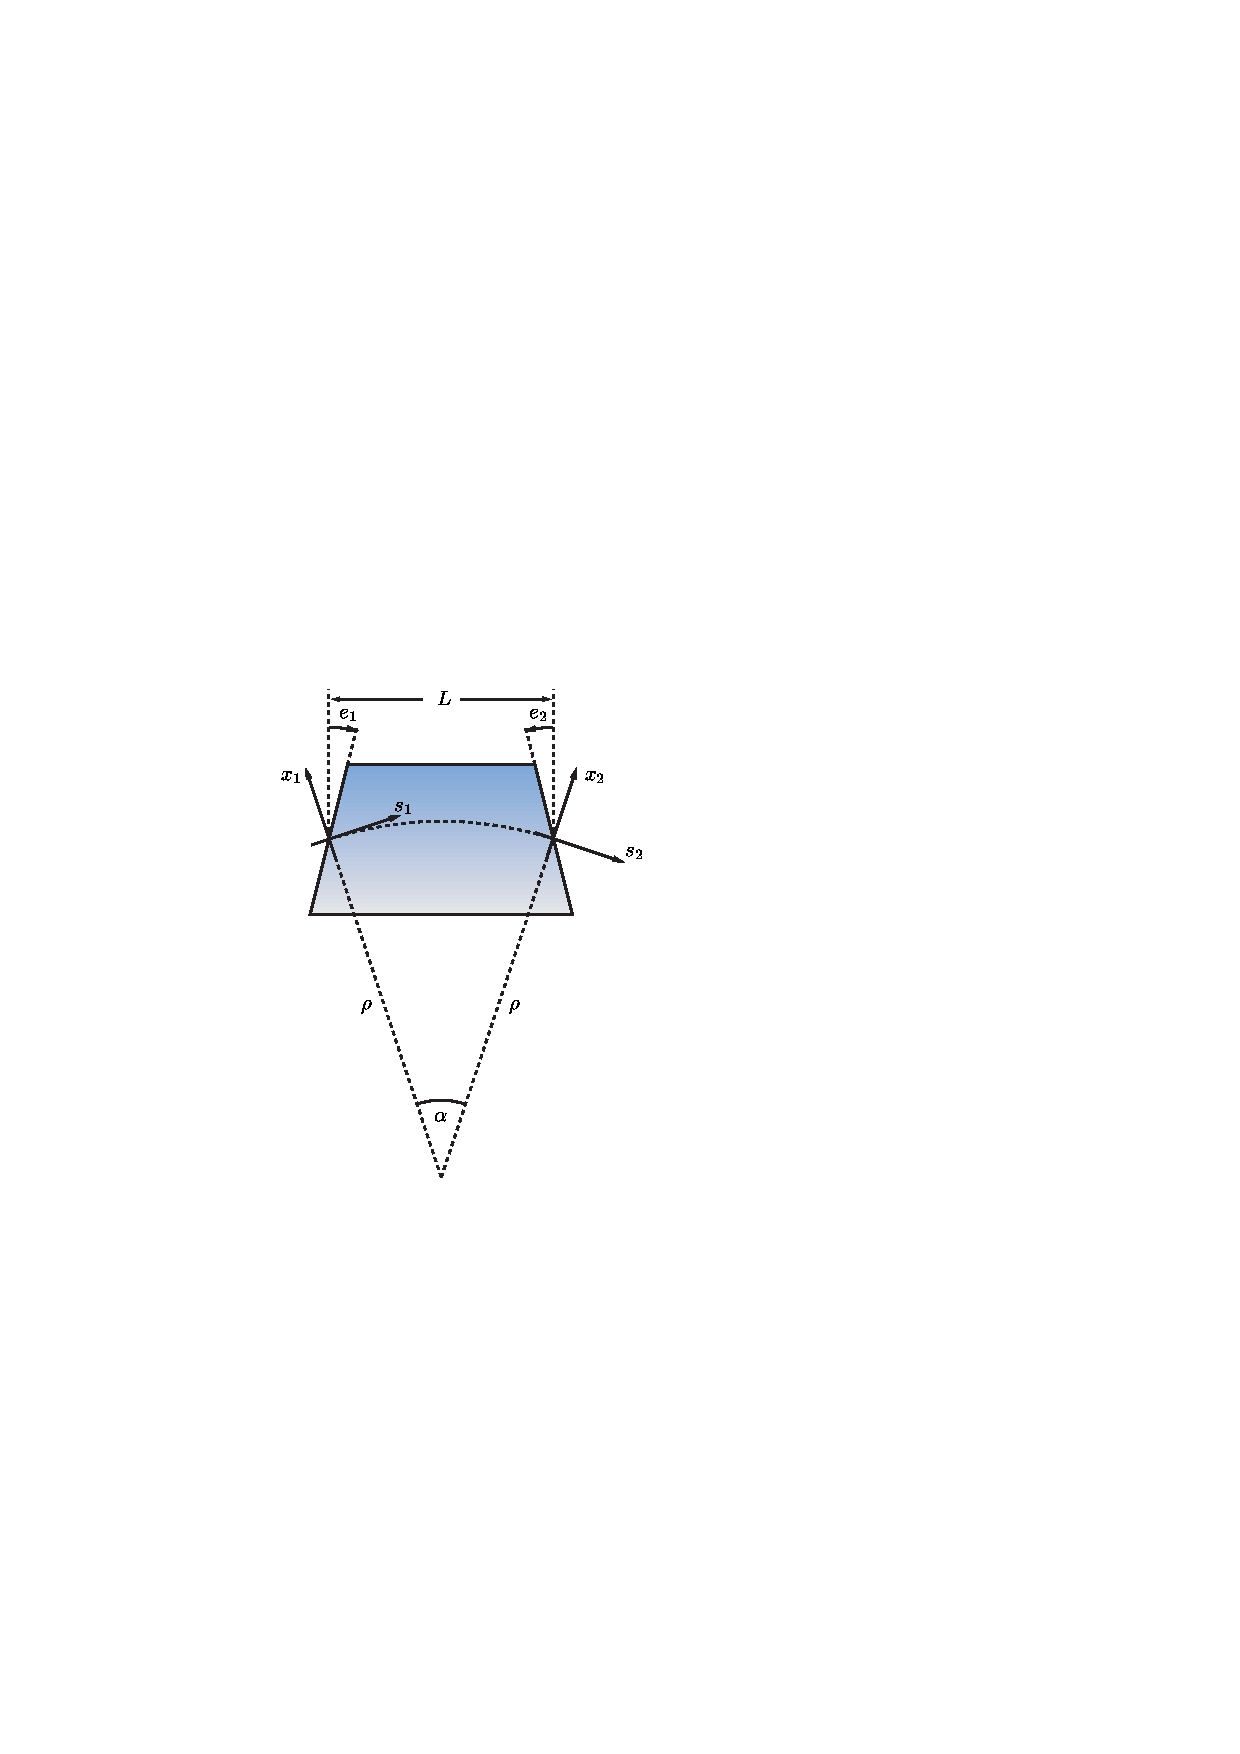
\includegraphics{rbend_coords.psfig}
    \label{rbend}
  }
  \hspace{1cm}
  \subfigure[sbend]
  {
    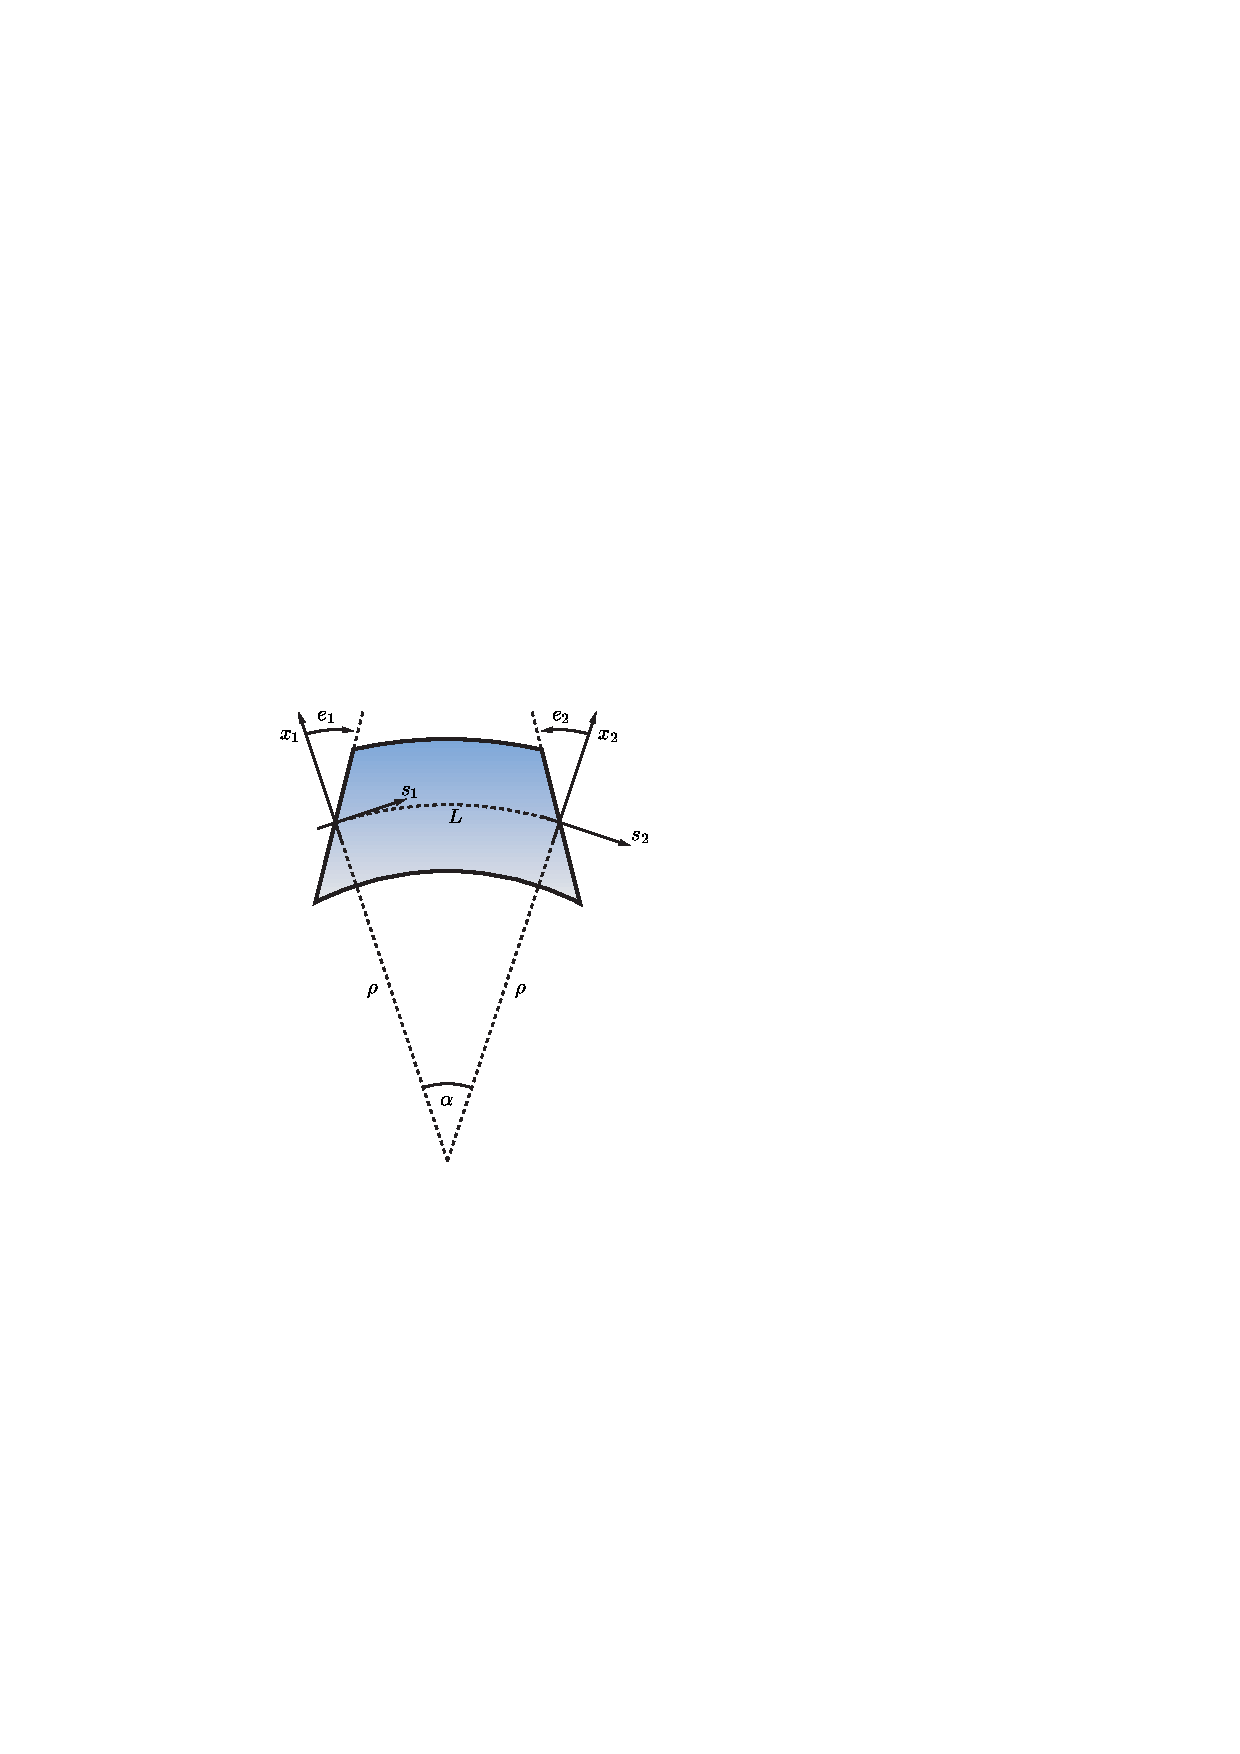
\includegraphics{sbend_coords.psfig}
    \label{sbend}
  }
  \caption{Coordinate systems for (a) \vn{Rbend}\ and (b) \vn{Sbend}\ 
  elements.}
\end{figure}

  \begin{description}
  \item[l]  
For a \vn{Rbend} \vn{l} is the chord length and not the arc length as
it is for a \vn{Sbend}.  After reading in a lattice, \bmad\ will
internally convert all \vn{Rbend}s into \vn{Sbend}s so internally
\vn{l} will become the path length. The chord length will be stored in
the \vn{l_chord} attribute.
  \item[h1, h2]
The attributes \vn{h1} and \vn{h2} are the curvature of the entrance
and exit pole faces. They are present for compatibility with MAD but
are not yet implemented in terms of tracking and other calculations.
  \item[e1, e2]
the rotation angle of the entrance pole face is \vn{e1} and at the exit
face it is \vn{e2}. An \vn{Sbend} with an \vn{e1} = \vn{e2} =
\vn{angle}/2 is equivalent to an \vn{Rbend} with \vn{e1} = \vn{e2} =
0.
  \item[angle]
The total design bend angle. A positive \vn{angle} represents a
bend towards negative $x$ values (see Figure~\ref{f:local_coords}).
  \item[k1]
The quadrupole strength.
  \item[g, delta\_g, rho]
The design bending radius which determines the reference coordinate
system is \vn{rho} (see section~\ref{s:ref}).  \vn{g} = 1/\vn{rho} is
the curvature function and is proportional to the design dipole
magnetic field. The true field strength is given by
\vn{g}~+~\vn{delta_g} so changing \vn{delta_g} leaves the design orbit
unchanged but varies a particle's orbit.
  \item[fint, fintx, hgap, hgapx]
The field integrals for the entrence and
exit pole faces are give by \vn{fint} and \vn{fintx} respectively
\Begineq
  F_{int} = \int_{pole} \! \! ds \, \frac{B_y(s) (B_0 - B_y(s))}
  {2 H_{gap} B_0^2}
\Endeq
with a similar equation for \vn{fintx}. \vn{hgap} and \vn{hgapx} are
the half gaps at the entrance and exit faces. If \vn{fint} or
\vn{fintx} is given without a value then a value of 0.5 is used. If
\vn{fint} or \vn{fintx} is not present then the default value of 0 is
used.
  \item[tilt]
The roll angle about the longitudinal axis at the entrence face of the
bend is given by \vn{tilt}.  \vn{tilt} = 0 bends the reference
trajectory in the $-x$ direction.  If the \vn{tilt} attribute is given
without any value then the value $\pi/2$ will be used. This makes for
a downward vertical ($-y$) bend.
  \end{description}


Note: \vn{g}, \vn{angle}, and \vn{l} are mutually dependent. If any two are
specified for an element \bmad\ will calculate the appropriate value
for the third.  After reading in a lattice, \vn{angle} is considered a
dependent variable.

Example:
\begin{example}
  b03w: sbend, l = 0.6, k1 = 0.003, fint  ! gives fint = 0.5, fintx = 0
\end{example}

%-----------------------------------------------------------------
\section{Collimators: Ecollimator and Rcollimator}
\label{s:col}
\index{Element!Ecollimator|textbf}
\index{Element!Rcollimator|textbf}

\begin{center}
\tt
\begin{tabular}{|l|l||l|l||l|l|} \hline
  {\sl Attribute} & {\sl Sec.}  & {\sl Attribute} & {\sl Sec.} & {\sl Attribute} & {\sl Sec.} \\ \hline
  l        = Real       & \ref{s:l}      & type = String    & \ref{s:string} & tracking\_method = Switch    & \ref{s:tkm}   \\ \hline
  num\_steps = Integer  & \ref{s:integ}  & alias = String   & \ref{s:string} & mat6\_calc\_method = Switch  & \ref{s:xfer}  \\ \hline
  rel\_tol = Real       & \ref{s:integ}  & descrip = String & \ref{s:string} & symplectify = Logical        & \ref{s:symp}  \\ \hline
  abs\_tol = Real       & \ref{s:integ}  & x\_limit = Real  & \ref{s:limit}  & integration\_ord = Integer   & \ref{s:integ} \\ \hline
  x\_offset  = Real     & \ref{s:offset} & y\_limit = Real  & \ref{s:limit}  & field\_calc = Switch         & \ref{s:integ} \\ \hline
  y\_offset  = Real     & \ref{s:offset} & aperture = Real  & \ref{s:limit}  & beam\_energy$^*$             & \ref{s:param} \\ \hline
                        &                &                  &                & aperture\_at = Switch        & \ref{s:limit} \\ \hline
  \multicolumn{6}{l}{\small $^*$Dependent attribute. See Chapter~\ref{c:attrib}} \\
\end{tabular}
\end{center}
\toffset

An \vn{Ecollimator} is a drift with elliptic collimation.
A \vn{Rcollimator} is a drift with rectangular collimation.
The aperture is considered to be at the end edge of the element.
Example:
\begin{example}
  d21: ecollimator, l = 4.5, x_limit = 0.09/2, y_limit = 0.05/2
\end{example}

%-----------------------------------------------------------------
\section{Custom}
\label{s:custom}
\index{Element!Custom|textbf}

\begin{center}
\tt
\begin{tabular}{|l|l||l|l||l|l|} \hline
  {\sl Attribute} & {\sl Sec.}  & {\sl Attribute} & {\sl Sec.}  & {\sl Attribute} & {\sl Sec.} \\ \hline
  l        = Real           & \ref{s:l}      & type = String    & \ref{s:string} & tracking\_method = Switch   & \ref{s:tkm}   \\ \hline
  val1,$\ldots$val12 = Real &                & alias = String   & \ref{s:string} & mat6\_calc\_method = Switch & \ref{s:xfer}  \\ \hline
  delta\_e   = Real         & \ref{s:offset} & descrip = String & \ref{s:string} & integration\_ord = Integer  & \ref{s:integ} \\ \hline
  x\_offset  = Real         & \ref{s:offset} & is\_on = Logical & \ref{s:is_on}  & field\_calc = Switch        & \ref{s:integ} \\ \hline
  y\_offset  = Real         & \ref{s:offset} & x\_limit = Real  & \ref{s:limit}  & rel\_tol = Real             & \ref{s:integ} \\ \hline
  s\_offset  = Real         & \ref{s:offset} & y\_limit = Real  & \ref{s:limit}  & abs\_tol = Real             & \ref{s:integ} \\ \hline
  x\_pitch = Real           & \ref{s:offset} & aperture = Real  & \ref{s:limit}  & num\_steps = Integer        & \ref{s:integ} \\ \hline
  y\_pitch = Real           & \ref{s:offset} &                  &                & symplectify = Logical       & \ref{s:symp}  \\ \hline
  tilt     = Real           & \ref{s:offset} & beam\_energy$^*$ & \ref{s:param}  & aperture\_at = Switch       & \ref{s:limit} \\ \hline
  \multicolumn{6}{l}{\small $^*$Dependent attribute. See Chapter~\ref{c:attrib}} \\
\end{tabular}
\end{center}
\toffset

A \vn{Custom} element is an element whose properties are defined
outside of the standard \bmad\ subroutine library. That is, to use a
custom element some programmer must write the appropriate custom
routines which are then linked with the \bmad\ subroutines into a
program. \bmad\ will call the custom routines at the appropriate time
to do tracking, transfer matrix calculations, etc. See the programmer
who wrote the custom routines for more details! See 
section~\ref{s:custom_ele} on how to write custom routines.

\vn{delta_e} is the energy gain of the {\it reference} particle
between the starting edge of the element and the ending edge.

Example:
\begin{example}
  c1: custom, l = 3, val4 = 5.6, val12 = 0.9, num_steps = 12, tracking_method = boris
\end{example}

%-----------------------------------------------------------------
\section{Drift}
\label{s:drift}
\index{Element!Drift|textbf}

\begin{center}
\tt
\begin{tabular}{|l|l||l|l||l|l|} \hline
  {\sl Attribute} & {\sl Sec.}  & {\sl Attribute} & {\sl Sec.} & {\sl Attribute} & {\sl Sec.} \\ \hline
  l        = Real       & \ref{s:l}     & type = String    & \ref{s:string} & tracking\_method = Switch    & \ref{s:tkm}   \\ \hline
                        &               & alias = String   & \ref{s:string} & mat6\_calc\_method = Switch  & \ref{s:xfer}  \\ \hline
  rel\_tol = Real       & \ref{s:integ} & descrip = String & \ref{s:string} &                              &               \\ \hline
  abs\_tol = Real       & \ref{s:integ} & x\_limit = Real  & \ref{s:limit}  & symplectify = Logical        & \ref{s:symp}  \\ \hline
  num\_steps = Integer  & \ref{s:integ} & y\_limit = Real  & \ref{s:limit}  & integration\_ord = Integer   & \ref{s:integ} \\ \hline
  beam\_energy$^*$      & \ref{s:param} & aperture = Real  & \ref{s:limit}  & field\_calc = Switch         & \ref{s:integ} \\ \hline
                        &               &                  &                & aperture\_at = Switch        & \ref{s:limit} \\ \hline
  \multicolumn{6}{l}{\small $^*$Dependent attribute. See Chapter~\ref{c:attrib}} \\
\end{tabular}
\end{center}
\toffset

A \vn{Drift} element is a space free and clear of any fields.
Example:
\begin{example}
  d21: drift, l = 4.5
\end{example}

%-----------------------------------------------------------------
\section{Elseparator}
\label{s:elsep}
\index{Element!Elseparator|textbf}

\begin{center}
\tt
\begin{tabular}{|l|l||l|l||l|l|} \hline
  {\sl Attribute} & {\sl Sec.}  & {\sl Attribute} & {\sl Sec.} & {\sl Attribute} & {\sl Sec.} \\ \hline
  l        = Real       & \ref{s:l}      & type = String    & \ref{s:string} & tracking\_method = Switch   & \ref{s:tkm}    \\ \hline
  hkick    = Real       & \ref{s:kick}   & alias = String   & \ref{s:string} & mat6\_calc\_method = Switch & \ref{s:xfer}   \\ \hline
  vkick    = Real       & \ref{s:kick}   & descrip = String & \ref{s:string} & integration\_ord = Integer  & \ref{s:integ}  \\ \hline
  gap      = Real       &                & is\_on = Logical & \ref{s:is_on}  & field\_calc = Switch        & \ref{s:integ}  \\ \hline
  x\_offset  = Real     & \ref{s:offset} & x\_limit = Real  & \ref{s:is_on}  & rel\_tol = Real             & \ref{s:integ}  \\ \hline
  y\_offset  = Real     & \ref{s:offset} & y\_limit = Real  & \ref{s:limit}  & abs\_tol = Real             & \ref{s:integ}  \\ \hline
  s\_offset  = Real     & \ref{s:offset} & aperture = Real  & \ref{s:limit}  & num\_steps = Integer        & \ref{s:integ}  \\ \hline
  x\_pitch = Real       & \ref{s:offset} &                  &                & symplectify = Logical       & \ref{s:symp}   \\ \hline
  y\_pitch = Real       & \ref{s:offset} & voltage$^*$      &                & a$n$, b$n$ = Real           & \ref{s:fields} \\ \hline
  tilt     = Real       & \ref{s:offset} & e\_field$^*$     &                & radius = Real               & \ref{s:fields} \\ \hline
                        &                & beam\_energy$^*$ & \ref{s:param}  & aperture\_at = Switch       & \ref{s:limit}  \\ \hline
  \multicolumn{6}{l}{\small $^*$Dependent attribute. See Chapter~\ref{c:attrib}} \\
\end{tabular}
\end{center}
\toffset

A \vn{ElSeparator} is an electrostatic separator.

For an \vn{Elseparator}, the kick is determined by \vn{hkick} and
\vn{vkick}. The \vn{gap} for an \vn{Elseparator} is used to compute
the electric field for a given kick. The voltage is a dependent
attribute determined by:
\begin{example}
  e\_field (V/m) = sqrt(hkick^2 + vkick^2) * beam\_energy / L
  voltage (V) = e\_field * gap  
\end{example}

Example:
\begin{example}
  h_sep: elsep, l = 4.5, hkick = 0.003, gap = 0.11
\end{example}

%-----------------------------------------------------------------
\section{Hkicker and Vkicker}
\label{s:hvkicker}
\index{Element!Hkicker|textbf}
\index{Element!Vkicker|textbf}

\begin{center}
\tt
\begin{tabular}{|l|l||l|l||l|l|} \hline
  {\sl Attribute} & {\sl Sec.} & {\sl Attribute} & {\sl Sec.} &  {\sl Attribute} & {\sl Sec.} \\ \hline
  l        = Real       & \ref{s:l}       & type = String    & \ref{s:string} & tracking\_method = Switch    & \ref{s:tkm}   \\ \hline
  kick     = Real       & \ref{s:kick}    & alias = String   & \ref{s:string} & mat6\_calc\_method = Switch  & \ref{s:xfer}  \\ \hline
  tilt     = Real       & \ref{s:offset}  & descrip = String & \ref{s:string} & integration\_ord = Integer   & \ref{s:integ} \\ \hline
  rel\_tol = Real       & \ref{s:integ}   & x\_limit = Real  & \ref{s:limit}  & field\_calc = Switch         & \ref{s:integ} \\ \hline 
  abs\_tol = Real       & \ref{s:integ}   & y\_limit = Real  & \ref{s:limit}  & symplectify = Logical        & \ref{s:symp}  \\ \hline
  num\_steps = Integer  & \ref{s:integ}   & aperture = Real  & \ref{s:limit}  & is\_on = Logical             & \ref{s:is_on} \\ \hline
  beam\_energy$^*$      & \ref{s:param}   &                  &                & aperture\_at = Switch        & \ref{s:limit} \\ \hline
  \multicolumn{6}{l}{\small $^*$Dependent attribute. See Chapter~\ref{c:attrib}} \\
\end{tabular}
\end{center}
\toffset

A \vn{Hkicker} is a horizontal bend and a \vn{Vkicker} is a vertical
bend.  Note that \vn{Hkicker} and \vn{Vkicker} elements use the
\vn{kick} attribute while a \vn{kicker} uses the \vn{hkick} and \vn{vkick} 
attributes. Example:
\begin{example}
  h_kick: hkicker, l = 4.5, kick = 0.003
\end{example}

%-----------------------------------------------------------------
\section{Hybrid}
\label{s:hybrid}
\index{Element!Hybrid|textbf}

A \vn{Hybrid} element is an element that is formed by concatenating
other element together. \vn{Hybrid} elements are not part of the input
lattice file but are created by a program, usually for speed purposes.

%-----------------------------------------------------------------
\section{I\_Beam}
\label{s:i_beam}
\index{Element!I_Beam|textbf}

\begin{center}
\tt
\begin{tabular}{|l|l||l|l||l|l|} \hline
  {\sl Attribute} & {\sl Sec.}  & {\sl Attribute} & {\sl Sec.} & {\sl Attribute} & {\sl Sec.} \\ \hline
  x\_offset  = Real     & \ref{s:offset}  &   x\_pitch  = Real     & \ref{s:offset}  &  type = String    & \ref{s:string}  \\ \hline
  y\_offset  = Real     & \ref{s:offset}  &   y\_pitch  = Real     & \ref{s:offset}  &  alias = String   & \ref{s:string}  \\ \hline
  s\_offset  = Real     & \ref{s:offset}  &   tilt      = Real     & \ref{s:offset}  &  descrip = String & \ref{s:string}  \\ \hline
  i\_beam = List        &                 &                        &                 &                   &                 \\ \hline
\end{tabular}
\end{center}
\toffset

An \vn{I_Beam} is a support structure that orients the elements that
are attached to it in space.

When an \vn{I_Beam} overlays an element, then that elements
orientation attributes (\vn{x_offset}, \vn{y_pitch}, \vn{tilt}, etc.) 
give the orientation of
the element with respect to the \vn{I_Beam}. An example will make this clear:
\begin{example}
  q1: quad, l = 10
  q2: quad, l = 5, x_offset = 0.2, x_pitch = 0.01
  ib: i_beam = \{q1, q2\}, x_pitch = 0.1, x_offset = 0.3
  this_line: line = (q1, q2)
  use, this
\end{example}
In this example \vn{ib} supports elements \vn{q1} and \vn{q2}. The
center of \vn{ib} is at $s = 7.5$ (\vn{ib} starts at $s = 0$ which is
the beginning of \vn{q1} and ends at $s = 15$ which is the end of
\vn{q2}). Like other elements, pitch is calculated from the center of
an \vn{I_Beam} element (see Sec.~\ref{s:offset}). The center of
\vn{q2} is at $s = 12.5$ so the distance between the center of \vn{ib}
and \vn{q2} is $ds = 5$. The pitch of \vn{ib} produces an offset at
the center of \vn{q2} of $0.5 = 0.1 * 5$. This, added to the offsets
of \vn{ib} and \vn{q2}, give the total offset of \vn{q2} to be $1.0 =
0.5 + 0.3 + 0.2$. The total \vn{x_pitch} of \vn{q2} is $0.11 = 0.1 +
0.01$. From the above example it can be seen that an \vn{I_Beam} looks
similar to an \vn{Overlay} (see Sec.~\ref{s:overlay}). It would,
however, take six \vn{Overlays} to simulate the effect of a single
\vn{I_Beam}.

The \vn{I_Beam} statement syntax is:
\begin{example}
  beam_name: I_BEAM = \{ele1, ele2, ... \}, ...
\end{example}
An \vn{I_Beam} element will be created for each \vn{ele1} element in
the lattice. The elements \vn{ele2}, \vn{ele3}, etc. do not have to be
consecutive but, if more than one \vn{I_Beam} is to be created, need
to be in order of increasing \vn{s}.
For example:
\begin{example}
  q1: quad
  q2: quad
  s0: sextupole
  s1: sextupole
  ib: i_beam = \{q1, s1, q2\}
  this_line: line = (q1, s0, s1, q2, ..., q1, s0, s1, q2)
  use, this
\end{example}
In this example two \vn{I_Beam} elements will be created.

Note to programmers: The total horizontal offset of any element is
stored in the element component \vn{%value(x_offset_tot\$)}. Similarly
the total tilt is stored in \vn{%value(tilt_tot\$)}, etc.

%-----------------------------------------------------------------
\section{Instrument and Monitor}
\label{s:monitor}
\index{Element!Instrument|textbf}
\index{Element!Monitor|textbf}

\begin{center}
\tt
\begin{tabular}{|l|l||l|l||l|l|} \hline
  {\sl Attribute} & {\sl Sec.}  & {\sl Attribute} & {\sl Sec.}  & {\sl Attribute} & {\sl Sec.} \\ \hline
  l        = Real       & \ref{s:l}     & type = String    & \ref{s:string} & tracking\_method = Switch    & \ref{s:tkm}   \\ \hline
                        &               & alias = String   & \ref{s:string} & mat6\_calc\_method = Switch  & \ref{s:xfer}  \\ \hline
  rel\_tol = Real       & \ref{s:integ} & descrip = String & \ref{s:string} & aperture\_at = Switch        & \ref{s:limit}  \\ \hline
  abs\_tol = Real       & \ref{s:integ} & x\_limit = Real  & \ref{s:limit}  & symplectify = Logical        & \ref{s:symp}  \\ \hline
  num\_steps = Integer  & \ref{s:integ} & y\_limit = Real  & \ref{s:limit}  & integration\_ord = Integer   & \ref{s:integ} \\ \hline
  beam\_energy$^*$      & \ref{s:param} & aperture = Real  & \ref{s:limit}  & field\_calc = Switch         & \ref{s:integ} \\ \hline
  \multicolumn{6}{l}{\small $^*$Dependent attribute. See Chapter~\ref{c:attrib}} \\
\end{tabular}
\end{center}
\toffset

\bmad\ treats \vn{Instrument} and \vn{Monitor} elements exactly like a
drift.  Example:
\begin{example}
  d21: instr, l = 4.5
\end{example}

%-----------------------------------------------------------------
\section{Kicker}
\label{s:kicker}
\index{Element!Kicker|textbf}

\begin{center}
\tt
\begin{tabular}{|l|l||l|l||l|l|} \hline
  {\sl Attribute} & {\sl Sec.} & {\sl Attribute} & {\sl Sec.}&  {\sl Attribute} & {\sl Sec.} \\ \hline
  l        = Real       & \ref{s:l}       & type = String    & \ref{s:string} & tracking\_method = Switch    & \ref{s:tkm}   \\ \hline
  hkick    = Real       & \ref{s:kick}    & alias = String   & \ref{s:string} & mat6\_calc\_method = Switch  & \ref{s:xfer}  \\ \hline
  vkick    = Real       & \ref{s:kick}    & descrip = String & \ref{s:string} & integration\_ord = Integer   & \ref{s:integ} \\ \hline
  h\_displace = Real    &                 & x\_limit = Real  & \ref{s:limit}  & field\_calc = Switch         & \ref{s:integ} \\ \hline 
  v\_displace = Real    &                 & y\_limit = Real  & \ref{s:limit}  & symplectify = Logical        & \ref{s:symp}  \\ \hline
  rel\_tol = Real       & \ref{s:integ}   & aperture = Real  & \ref{s:limit}  & is\_on = Logical             & \ref{s:is_on} \\ \hline
  abs\_tol = Real       & \ref{s:integ}   &                  &                & aperture\_at = Switch        & \ref{s:limit} \\ \hline
  num\_steps = Integer  & \ref{s:integ}   & tilt     = Real  & \ref{s:offset} & beam\_energy$^*$             & \ref{s:param} \\ \hline
  \multicolumn{6}{l}{\small $^*$Dependent attribute. See Chapter~\ref{c:attrib}} \\
\end{tabular}
\end{center}
\toffset

A \vn{Kicker} can deflect a beam in both planes. Note that a
\vn{Kicker} uses the \vn{hkick} and \vn{vkick} attributes while
\vn{Hkicker} and \vn{Vkicker} elements use the \vn{kick} attribute. 
In addition a \vn{Kicker} can apply a displacement to a particle
using the \vn{h_displace} and \vn{v_displace} attributes.
Example:
\begin{example}
  a_kick: kicker, l = 4.5, hkick = 0.003
\end{example}

%-----------------------------------------------------------------
\section{Lcavity}
\label{s:lcav}
\index{Element!Lcavity|textbf}

\begin{center}
\tt
\begin{tabular}{|l|l||l|l||l|l|} \hline
  {\sl Attribute} & {\sl Sec.}  & {\sl Attribute} & {\sl Sec.} & {\sl Attribute} & {\sl Sec.} \\ \hline
  l        = Real       & \ref{s:l}      & type = String     & \ref{s:string} & tracking\_method = Switch   & \ref{s:tkm}   \\ \hline
  rf\_frequency = Real  &                & alias = String    & \ref{s:string} & mat6\_calc\_method = Switch & \ref{s:xfer}  \\ \hline
  gradient      = Real  &                & descrip = String  & \ref{s:string} & integration\_ord = Integer  & \ref{s:integ} \\ \hline
  phi0          = Real  &                & is\_on = Logical  & \ref{s:is_on}  & field\_calc = Switch        & \ref{s:integ} \\ \hline
  e\_loss       = Real  &                & x\_limit = Real   & \ref{s:limit}  & rel\_tol = Real             & \ref{s:integ} \\ \hline
  x\_offset  = Real     & \ref{s:offset} & y\_limit = Real   & \ref{s:limit}  & abs\_tol = Real             & \ref{s:integ} \\ \hline
  y\_offset  = Real     & \ref{s:offset} & aperture = Real   & \ref{s:limit}  & num\_steps = Integer        & \ref{s:integ} \\ \hline
  s\_offset  = Real     & \ref{s:offset} & hkick    = Real   & \ref{s:kick}   & lr\_wake\_file = String     &               \\ \hline
  x\_pitch = Real       & \ref{s:offset} & vkick    = Real   & \ref{s:kick}   & sr\_wake\_file = String     &               \\ \hline
  y\_pitch = Real       & \ref{s:offset} & energy\_start$^*$ &                & aperture\_at = Switch       & \ref{s:limit} \\ \hline
  beam\_energy$^*$      & \ref{s:param}  & e\_loss$^*$       &                & delta\_e$^*$                &               \\ \hline
  \multicolumn{6}{l}{\small $^*$Dependent attribute. See Chapter~\ref{c:attrib}} \\
\end{tabular}
\end{center}
\toffset

\index{Lattice files!primary}
An \vn{Lcavity} is a LINAC accelerating cavity.
Tracking through an \vn{Lcavity} is modeled using the equations
developed by Rosenzweig and Serafini\cite{b:rosenzweig}. The
attributes specific to an \vn{Lcavity} are The dependent variable
\vn{delta_e} attribute can be used in place of \vn{gradient} in a
primary lattice file as discussed in Section~\ref{s:depend}.
\begin{example}
  gradient     ! Accelerating gradient (V/m).
  phi0         ! Phase (radians/2\(\pi\)) of the reference particle with 
               !   respect to the RF. phi0 = 0 is on crest.
  e_loss       ! Loss parameter for short range wakefields (V/Coulomb).
  rf_frequency ! Rf frequency (Hz).
  sr_wake_file ! Short range wake field definition file.
  lr_wake_file ! Long range wake field definition file.
\end{example}

The kick felt by a particle is 
\begin{example}
  dE = gradient * L * cos(twopi * (phi0 - z * rf_frequency / c_light))
\end{example}
This is consistent with MAD and LIAR. Note: The MAD8 documentation 
for an \vn{Lcavity} gives essentially
\begin{example}
  dE = gradient * L * cos(twopi * (phi0 + z * rf_frequency / c_light)) ! WRONG
\end{example}
This is incorrect.

Note: The transfer matrix for an \vn{Lcavity} with finite
\vn{gradient} is never symplectic.

Example:
\begin{example}
  rf1: lcav, l = 4.5, gradient = 1.2e6, sr\_wake\_file = "sr1.dat"
\end{example}

The input file name for the short--range wakefields is specified using the 
\vn{sr_wake_file} attribute. The file gives both longitudinal and transverse wakes in 
tabular form. Comment header lines may be included by starting a line
with an exclamation mark (!) or by leaving the line blank. 
An example input file is:
\begin{example}
!    z[m]       Wz[V/C/m]   Wt[V/C/m^2]

 0.00000E+00  1.61125E+15   0.00000E+00     1 
 1.00000E-05  1.44516E+15   1.30560E+15     2 
 2.00000E-05  1.38148E+15   2.50665E+15     3 
 ... etc ...
 1.97000E-03  3.49958E+14   7.95507E+16   198 
 1.98000E-03  3.48606E+14   7.97253E+16   199 
 1.99000E-03  3.47263E+14   7.98989E+16   200 
\end{example}
The first column is the longitudinal distance $z$. $z$ must start at 0 and must increment by
the a constant amount from row to row. The second column is the longitudinal wake function in
$V/C/m$. The third column is the transverse wake in $V/C/m^2$. Any additional columns are ignored.

Note:  \vn{e_loss} is only a dependent varif a \vn{sr_wake_file} is present. In this case
it is computed from the $z = 0$ longitudinal wake. 

\vn{delta_e} is simply defined to be
\begin{example}
  delta_e = gradient * L
\end{example}


%-----------------------------------------------------------------
\section{Marker}
\label{s:mark}
\index{Element!Marker|textbf}

\begin{center}
\tt
\begin{tabular}{|l|l||l|l||l|l|} \hline
  {\sl Attribute} & {\sl Sec.}  & {\sl Attribute} & {\sl Sec.} & {\sl Attribute} & {\sl Sec.} \\ \hline
  tracking\_method = Switch    & \ref{s:tkm}  &  type = String      & \ref{s:string} & x\_limit = Real       & \ref{s:limit} \\ \hline 
  mat6\_calc\_method = Switch  & \ref{s:xfer} &  alias = String     & \ref{s:string} & y\_limit = Real       & \ref{s:limit} \\ \hline 
  beam\_energy$^*$             & \ref{s:param}&  descrip = String   & \ref{s:string} & aperture = Real       & \ref{s:limit} \\ \hline 
                               &              &                     &                & aperture\_at = Switch & \ref{s:limit} \\ \hline
  \multicolumn{6}{l}{\small $^*$Dependent attribute. See Chapter~\ref{c:attrib}} \\
\end{tabular}
\end{center}
\toffset

A \vn{Marker} is a zero length element meant to mark a position.
Example:
\begin{example}
  mm: mark, type = "BPM"
\end{example}

%-----------------------------------------------------------------
\section{Match}
\label{s:match}
\index{Element!Match|textbf}

\begin{center}
\tt
\begin{tabular}{|l|l||l|l||l|l|} \hline
  {\sl Attribute} & {\sl Sec.}  & {\sl Attribute} & {\sl Sec.} & {\sl Attribute} & {\sl Sec.} \\ \hline
  beta\_x0  = Real &               & beta\_x1  = Real &               & tracking\_method = Switch   & \ref{s:tkm}    \\ \hline
  alpha\_x0 = Real &               & alpha\_x1 = Real &               & mat6\_calc\_method = Switch & \ref{s:xfer}   \\ \hline
  eta\_x0   = Real &               & eta\_x1   = Real &               & x\_limit = Real             & \ref{s:limit}  \\ \hline
  etap\_x0  = Real &               & etap\_x1  = Real &               & y\_limit = Real             & \ref{s:limit}  \\ \hline
  beta\_y0  = Real &               & beta\_y1  = Real &               & aperture = Real             & \ref{s:limit}  \\ \hline
  alpha\_y0 = Real &               & alpha\_y1 = Real &               & aperture\_at = Switch       & \ref{s:limit}  \\ \hline
  eta\_y0   = Real &               & eta\_y1   = Real &               & type = String               & \ref{s:string} \\ \hline
  etap\_y0  = Real &               & etap\_y1  = Real &               & alias = String              & \ref{s:string} \\ \hline
  dphi\_x   = Real &               & beam\_energy$^*$ & \ref{s:param} & descrip = String            & \ref{s:string} \\ \hline
  dphi\_y   = Real &               &                  &               & is\_on = Logical            & \ref{s:is_on}  \\ \hline
  \multicolumn{6}{l}{\small $^*$Dependent attribute. See Chapter~\ref{c:attrib}} \\
\end{tabular}
\end{center}
\toffset

A \vn{Match} element is used to match the Twiss parameters between two points. That is, 
the tranfer map for a match element, which is just a linear matrix, is calculated such that
if the Twiss parameters at the exit end of the element preceding the \vn{match} element are 
given by \vn{beta_x0}, \vn{beta_y0}, etc., then the computed Twiss parameters at the exit
end of the \vn{match} element will be \vn{beta_x1}, \vn{beta_y1}, etc. \vn{dphi_x} and \vn{dphi_y}
are the phase advances in radians.

Example:
\begin{example}
  mm: match, beta_x0 = 12.5, beta_y0 = 3.4, eta_x0 = 1.0, ...
\end{example}

%-----------------------------------------------------------------
\section{Multipole}
\label{s:mult}
\index{Element!Multipole|textbf}

\begin{center}
\tt
\begin{tabular}{|l|l||l|l||l|l|} \hline
  {\sl Attribute} & {\sl Sec}  & {\sl Attribute} & {\sl Sec} & {\sl Attribute} & {\sl Sec} \\ \hline
  K$n$L, T$n$ = Real &  \ref{s:fields} &  type = String       & \ref{s:string} & tracking\_method = Switch   & \ref{s:tkm}   \\ \hline
  tilt       = Real  &  \ref{s:offset} &  alias = String      & \ref{s:string} & mat6\_calc\_method = Switch & \ref{s:xfer}  \\ \hline
  x\_offset  = Real  &  \ref{s:offset} &  descrip = String    & \ref{s:string} & x\_limit = Real             & \ref{s:limit} \\ \hline
  y\_offset  = Real  &  \ref{s:offset} &  is\_on = Logical    & \ref{s:is_on}  & y\_limit = Real             & \ref{s:limit} \\ \hline
  s\_offset  = Real  &  \ref{s:offset} &  beam\_energy$^*$    & \ref{s:param}  & aperture = Real             & \ref{s:limit} \\ \hline
                     &                 &                      &                & aperture\_at = Switch       & \ref{s:limit} \\ \hline
  \multicolumn{6}{l}{\small $^*$Dependent attribute. See Chapter~\ref{c:attrib}} \\
\end{tabular}
\end{center}
\toffset

A \vn{Multipole} is a thin multipole lens up to 20th order. The only
difference between this and an \vn{AB_Multipole} is the input format. See the 
Magnetic fields section \ref{s:fields} for more details.

Like a \mad\ \vn{multipole}, A \bmad \vn{Multipole} will affect the
reference orbit if there is a dipole component. 
Example:
\begin{example}
  m1: multipole, k1l = 0.034e-2, t1, k3l = 4.5, t3 = 0.31*pi
\end{example}

%-----------------------------------------------------------------
\section{Octupole}
\label{s:oct}
\index{Element!Octupole|textbf}

\begin{center}
\tt
\begin{tabular}{|l|l||l|l||l|l|} \hline
  {\sl Attribute} & {\sl Sec.}  & {\sl Attribute} & {\sl Sec.} & {\sl Attribute} & {\sl Sec.} \\ \hline
  l        = Real        & \ref{s:l}      & type = String     & \ref{s:string} & tracking\_method = Switch   & \ref{s:tkm}    \\ \hline
  k3\DAG   = Real        &                & alias = String    & \ref{s:string} & mat6\_calc\_method = Switch & \ref{s:xfer}   \\ \hline
  b\_gradient\DAG = Real &                & descrip = String  & \ref{s:string} & integration\_ord = Integer  & \ref{s:integ}  \\ \hline
  x\_offset  = Real      & \ref{s:offset} & is\_on = Logical  & \ref{s:is_on}  & field\_calc = Switch        & \ref{s:integ}  \\ \hline
  y\_offset  = Real      & \ref{s:offset} & x\_limit = Real   & \ref{s:limit}  & rel\_tol = Real             & \ref{s:integ}  \\ \hline
  s\_offset  = Real      & \ref{s:offset} & y\_limit = Real   & \ref{s:limit}  & abs\_tol = Real             & \ref{s:integ}  \\ \hline
  x\_pitch = Real        & \ref{s:offset} & aperture = Real   & \ref{s:limit}  & num\_steps = Integer        & \ref{s:integ}  \\ \hline
  y\_pitch = Real        & \ref{s:offset} & a$n$, b$n$ = Real & \ref{s:fields} & radius = Real               & \ref{s:fields} \\ \hline
  tilt                   & \ref{s:offset} & hkick    = Real   & \ref{s:kick}   & symplectify = Logical       & \ref{s:symp}   \\ \hline
  beam\_energy$^*$       & \ref{s:param}  & vkick    = Real   & \ref{s:kick}   & aperture\_at = Switch       & \ref{s:limit}  \\ \hline
  \multicolumn{6}{l}{\small $^*$Dependent attribute. \DAG May be a dependent attribute. See Chapter~\ref{c:attrib}} \\
\end{tabular}
\end{center}
\toffset

An \vn{Octupole} has a cubic field dependence.
The \vn{Bmad_Standard} calculation treats an octupole using a kick--drift--kick model.

If the \vn{tilt} attribute is present without a value then a value of 
$\pi/8$ is used.
Example:
\begin{example}
  oct1: octupole, l = 4.5, k3 = 0.003, tilt ! same as tilt = pi/8
\end{example}

%-----------------------------------------------------------------
\section{Patch}
\label{s:patch}
\index{Element!Patch|textbf}

\begin{center}
\tt
\begin{tabular}{|l|l||l|l||l|l|} \hline
  {\sl Attribute} & {\sl Sec}  & {\sl Attribute} & {\sl Sec} & {\sl Attribute} & {\sl Sec} \\ \hline
  x\_offset  = Real  & \ref{s:offset} &  type = String      & \ref{s:string} & tracking\_method = Switch   & \ref{s:tkm}   \\ \hline
  y\_offset  = Real  & \ref{s:offset} &  alias = String     & \ref{s:string} & mat6\_calc\_method = Switch & \ref{s:xfer}  \\ \hline
  z\_offset  = Real  & \ref{s:offset} &  descrip = String   & \ref{s:string} & x\_limit = Real             & \ref{s:limit} \\ \hline
  tilt = Real        & \ref{s:offset} &  x\_pitch   = Real  & \ref{s:offset} & y\_limit = Real             & \ref{s:limit} \\ \hline
  de\_offset = Real  &                &  y\_pitch   = Real  & \ref{s:offset} & aperture = Real             & \ref{s:limit} \\ \hline
  beam\_energy$^*$   & \ref{s:param}  &  is\_on = Logical   & \ref{s:is_on}  & aperture\_at = Switch       & \ref{s:limit} \\ \hline
  \multicolumn{6}{l}{\small $^*$Dependent attribute. See Chapter~\ref{c:attrib}} \\
\end{tabular}
\end{center}
\toffset

A \vn{Patch} offsets the reference orbit. This is a generalization of
\mad's \vn{yrot} and \vn{srot} elements. For example, a positive
\vn{x_offset} offsets the reference orbit after the \vn{patch} in the
positive $x$--direction relative to the reference orbit before the
\vn{patch}.
Example:
\begin{example}
  pt: patch, x\_offset = 3.2
\end{example}

%-----------------------------------------------------------------
\section{Quadrupole}
\label{s:quad}
\index{Element!Quadrupole|textbf}

\begin{center}
\tt
\begin{tabular}{|l|l||l|l||l|l|} \hline
  {\sl Attribute} & {\sl Sec.}  & {\sl Attribute} & {\sl Sec.} & {\sl Attribute} & {\sl Sec.} \\ \hline
  l        = Real        & \ref{s:l}      & type = String      & \ref{s:string} & tracking\_method = Switch   & \ref{s:tkm}   \\ \hline
  k1\DAG   = Real        &                & alias = String     & \ref{s:string} & mat6\_calc\_method = Switch & \ref{s:xfer}  \\ \hline
  b\_gradient\DAG = Real &                & descrip = String   & \ref{s:string} & integration\_ord = Integer  & \ref{s:integ} \\ \hline
                         &                & is\_on = Logical   & \ref{s:is_on}  & field\_calc = Switch        & \ref{s:integ} \\ \hline
  x\_offset  = Real      & \ref{s:offset} & x\_limit = Real    & \ref{s:limit}  & rel\_tol = Real             & \ref{s:integ} \\ \hline
  y\_offset  = Real      & \ref{s:offset} & y\_limit = Real    & \ref{s:limit}  & abs\_tol = Real             & \ref{s:integ} \\ \hline
  s\_offset  = Real      & \ref{s:offset} & aperture = Real    & \ref{s:limit}  & num\_steps = Integer        & \ref{s:integ} \\ \hline
  x\_pitch = Real        & \ref{s:offset} & hkick    = Real    & \ref{s:kick}   & a$n$, b$n$ = Real           & \ref{s:fields}\\ \hline
  y\_pitch = Real        & \ref{s:offset} & vkick    = Real    & \ref{s:kick}   & radius = Real               & \ref{s:fields}\\ \hline
  tilt     = Real        & \ref{s:offset} & beam\_energy$^*$   & \ref{s:param}  & symplectify = Logical       & \ref{s:symp}  \\ \hline
                         &                &                    &                & aperture\_at = Switch       & \ref{s:limit} \\ \hline
  \multicolumn{6}{l}{\small $^*$Dependent attribute. \DAG May be a dependent attribute. See Chapter~\ref{c:attrib}} \\
\end{tabular}
\end{center}
\toffset

A \vn{Quadrupole} has a linear field dependence.
If the \vn{tilt} attribute is present without a value then a value of $\pi/4$
is used.
Example:
\begin{example}
  q03w: quad, l = 0.6, k1 = 0.003, tilt  ! same as tilt = pi/4
\end{example}

%-----------------------------------------------------------------
\section{RFcavity}
\label{s:rfcav}
\index{Element!RFcavity|textbf}

\begin{center}
\tt
\begin{tabular}{|l|l||l|l||l|l|} \hline
  {\sl Attribute} & {\sl Sec.}  & {\sl Attribute} & {\sl Sec.} & {\sl Attribute} & {\sl Sec.} \\ \hline
  l        = Real     & \ref{s:l}      & type = String      & \ref{s:string} & tracking\_method = Switch   & \ref{s:tkm}   \\ \hline
  harmon   = Real     &                & alias = String     & \ref{s:string} & mat6\_calc\_method = Switch & \ref{s:xfer}  \\ \hline
  voltage  = Real     &                & descrip = String   & \ref{s:string} & integration\_ord = Integer  & \ref{s:integ} \\ \hline
  phi0     = Real     &                & rf\_frequency = Real &              & field\_calc = Switch        & \ref{s:integ} \\ \hline
  x\_offset  = Real   & \ref{s:offset} & x\_limit = Real    & \ref{s:limit}  & rel\_tol = Real             & \ref{s:integ} \\ \hline
  y\_offset  = Real   & \ref{s:offset} & y\_limit = Real    & \ref{s:limit}  & abs\_tol = Real             & \ref{s:integ} \\ \hline
  s\_offset  = Real   & \ref{s:offset} & aperture = Real    & \ref{s:limit}  & num\_steps = Integer        & \ref{s:integ} \\ \hline
  x\_pitch = Real     & \ref{s:offset} & hkick    = Real    & \ref{s:kick}   & is\_on = Logical            & \ref{s:is_on} \\ \hline
  y\_pitch = Real     & \ref{s:offset} & vkick    = Real    & \ref{s:kick}   & symplectify = Logical       & \ref{s:symp}  \\ \hline
  beam\_energy$^*$    & \ref{s:param}  &                    &                & aperture\_at = Switch       & \ref{s:limit} \\ \hline
  \multicolumn{6}{l}{\small $^*$Dependent attribute. See Chapter~\ref{c:attrib}} \\
\end{tabular}
\end{center}
\toffset

An \vn{RFcavity} is an RF cavity without acceleration generally used
in a storage ring.

The \vn{phi0} attribute here is identical to the \vn{lag} attribute of
MAD. The kick felt by a particle is 
\begin{example}
  dE = voltage * sin(twopi * (phi0 + z * rf_frequency / c_light))
\end{example}
If \vn{harmon} is non--zero then \vn{rf_frequency} is a dependent
attribute calculated by
\begin{example}
  rf_frequency = harmon * c_light / L_lattice 
\end{example}
where \vn{L_lattice} is the total lattice length.

Example:
\begin{example}
  rf1: rfcav, l = 4.5, harmon = 1281, voltage = 5e6
\end{example}

%-----------------------------------------------------------------
\section{Sextupole}
\label{s:sex}
\index{Element!Sextupole|textbf}

\begin{center}
\tt
\begin{tabular}{|l|l||l|l||l|l|} \hline
  {\sl Attribute} & {\sl Sec.}  & {\sl Attribute} & {\sl Sec.} & {\sl Attribute} & {\sl Sec.} \\ \hline
  l        = Real        & \ref{s:l}      & type = String      & \ref{s:string} & tracking\_method = Switch   & \ref{s:tkm}   \\ \hline
  k2\DAG   = Real        &                & alias = String     & \ref{s:string} & mat6\_calc\_method = Switch & \ref{s:xfer}  \\ \hline
  b\_gradient\DAG = Real &                & descrip = String   & \ref{s:string} & integration\_ord = Integer  & \ref{s:integ} \\ \hline
  x\_offset  = Real      & \ref{s:offset} & is\_on = Logical   & \ref{s:is_on}  & field\_calc = Switch        & \ref{s:integ} \\ \hline
  y\_offset  = Real      & \ref{s:offset} & x\_limit = Real    & \ref{s:limit}  & rel\_tol = Real             & \ref{s:integ} \\ \hline
  s\_offset  = Real      & \ref{s:offset} & y\_limit = Real    & \ref{s:limit}  & abs\_tol = Real             & \ref{s:integ} \\ \hline
  x\_pitch = Real        & \ref{s:offset} & aperture = Real    & \ref{s:limit}  & num\_steps = Integer        & \ref{s:integ} \\ \hline
  y\_pitch = Real        & \ref{s:offset} & hkick    = Real    & \ref{s:kick}   & aperture\_at = Switch       & \ref{s:limit} \\ \hline
  tilt     = Real        & \ref{s:offset} & vkick    = Real    & \ref{s:kick}   & radius = Real               & \ref{s:fields}\\ \hline
  beam\_energy$^*$       & \ref{s:param}  & a$n$, b$n$ = Real  & \ref{s:fields} & symplectify = Logical       & \ref{s:symp}  \\ \hline
  \multicolumn{6}{l}{\small $^*$Dependent attribute. \DAG May be a dependent attribute. See Chapter~\ref{c:attrib}} \\
\end{tabular}
\end{center}
\toffset

A \vn{Sextupole} is an element with a magnetic field that varies quadratically with transverse offset. The \vn{Bmad_Standard} calculation treats a sextupole using a kick--drift--kick model.

If the \vn{tilt} attribute is present without a value then a value of 
$\pi/6$ is used.
Example:
\begin{example}
  q03w: quad, l = 0.6, k1 = 0.003, tilt  ! same as tilt = pi/6
\end{example}

%-----------------------------------------------------------------
\section{Solenoid}
\label{s:sol}
\index{Element!Solenoid|textbf}

\begin{center}
\tt
\begin{tabular}{|l|l||l|l||l|l|} \hline
  {\sl Attribute} & {\sl Sec.}  & {\sl Attribute} & {\sl Sec.} & {\sl Attribute} & {\sl Sec.} \\ \hline
  l        = Real        & \ref{s:l}      & type = String      & \ref{s:string} & tracking\_method = Switch   & \ref{s:tkm}   \\ \hline
  ks\DAG   = Real        &                & alias = String     & \ref{s:string} & mat6\_calc\_method = Switch & \ref{s:xfer}  \\ \hline
  b\_gradient\DAG = Real &                & descrip = String   & \ref{s:string} & integration\_ord = Integer  & \ref{s:integ} \\ \hline
                         &                & is\_on = Logical   & \ref{s:is_on}  & field\_calc = Switch        & \ref{s:integ} \\ \hline
  x\_offset  = Real      & \ref{s:offset} & x\_limit = Real    & \ref{s:limit}  & rel\_tol = Real             & \ref{s:integ} \\ \hline
  y\_offset  = Real      & \ref{s:offset} & y\_limit = Real    & \ref{s:limit}  & abs\_tol = Real             & \ref{s:integ} \\ \hline
  s\_offset  = Real      & \ref{s:offset} & aperture = Real    & \ref{s:limit}  & num\_steps = Integer        & \ref{s:integ} \\ \hline
  x\_pitch = Real        & \ref{s:offset} & hkick    = Real    & \ref{s:kick}   & aperture\_at = Switch       & \ref{s:limit} \\ \hline
  y\_pitch = Real        & \ref{s:offset} & vkick    = Real    & \ref{s:kick}   & radius = Real               & \ref{s:fields}\\ \hline
  beam\_energy$^*$       & \ref{s:param}  & a$n$, b$n$ = Real  & \ref{s:fields} & symplectify = Logical       & \ref{s:symp}  \\ \hline
  \multicolumn{6}{l}{\small $^*$Dependent attribute. \DAG May be a dependent attribute. See Chapter~\ref{c:attrib}} \\
\end{tabular}
\end{center}
\toffset

A \vn{Solenoid} is an element with a longitidinal magnetic field.
Example:
\begin{example}
  cleo_sol: solenoid, l = 2.6, ks = 1.5*beam[energy]
\end{example}

%-----------------------------------------------------------------
\section{Sol\_Quad}
\label{s:sq}
\index{Element!Sol_Quad|textbf}

\begin{center}
\tt
\begin{tabular}{|l|l||l|l||l|l|} \hline
  {\sl Attribute} & {\sl Sec.}  & {\sl Attribute} & {\sl Sec.} & {\sl Attribute} & {\sl Sec.} \\ \hline
  l        = Real     & \ref{s:l}      & type = String     & \ref{s:string} & tracking\_method = Switch   & \ref{s:tkm}   \\ \hline
  ks\DAG   = Real     &                & alias = String    & \ref{s:string} & mat6\_calc\_method = Switch & \ref{s:xfer}  \\ \hline
  k1       = Real     &                & descrip = String  & \ref{s:string} & integration\_ord = Integer  & \ref{s:integ} \\ \hline
  b\_field\DAG = Real &                & is\_on = Logical  & \ref{s:is_on}  & field\_calc = Switch        & \ref{s:integ} \\ \hline
  x\_offset  = Real   & \ref{s:offset} & x\_limit = Real   & \ref{s:limit}  & rel\_tol = Real             & \ref{s:integ} \\ \hline
  y\_offset  = Real   & \ref{s:offset} & y\_limit = Real   & \ref{s:limit}  & abs\_tol = Real             & \ref{s:integ} \\ \hline
  s\_offset  = Real   & \ref{s:offset} & aperture = Real   & \ref{s:limit}  & num\_steps = Integer        & \ref{s:integ} \\ \hline
  x\_pitch = Real     & \ref{s:offset} & hkick    = Real   & \ref{s:kick}   & a$n$, b$n$ = Real           & \ref{s:fields}\\ \hline
  y\_pitch = Real     & \ref{s:offset} & vkick    = Real   & \ref{s:kick}   & radius = Real               & \ref{s:fields}\\ \hline
  tilt     = Real     & \ref{s:offset} & beam\_energy$^*$  & \ref{s:param}  & symplectify = Logical       & \ref{s:symp}  \\ \hline
                      &                &                   &                & aperture\_at = Switch       & \ref{s:limit} \\ \hline
  \multicolumn{6}{l}{\small $^*$Dependent attribute. \DAG May be a dependent attribute. See Chapter~\ref{c:attrib}} \\
\end{tabular}
\end{center}
\toffset

A \vn{Sol_Quad} is a combination solenoid/quadrupole.
Example:
\begin{example}
  sq02: sol_quad, l = 2.6, k1 = 0.632, ks = 1.5*beam[energy]
\end{example}

%-----------------------------------------------------------------
\section{Taylor}
\label{s:tay}
\index{Element!Taylor|textbf}

\begin{center}
\tt
\begin{tabular}{|l|l||l|l||l|l|} \hline
  {\sl Attribute} & {\sl Sec.}  & {\sl Attribute} & {\sl Sec.} & {\sl Attribute} & {\sl Sec.} \\ \hline
  $\{ \tt \mbox{out:}\,  coef, \, e1 \, e2 \, e3 \, e4 \, e5 \, e6 \}$ 
                              &              & type = String    & \ref{s:string} & x\_limit = Real       & \ref{s:limit} \\ \hline  
  tracking\_method = Switch   & \ref{s:tkm}  & alias = String   & \ref{s:string} & y\_limit = Real       & \ref{s:limit} \\ \hline
  mat6\_calc\_method = Switch & \ref{s:xfer} & descrip = String & \ref{s:string} & aperture = Real       & \ref{s:limit} \\ \hline
  symplectify = Logical       & \ref{s:symp} & beam\_energy$^*$ & \ref{s:param}  & is\_on = Logical      & \ref{s:is_on} \\ \hline
                              &              &                  &                & aperture\_at = Switch & \ref{s:limit} \\ \hline
  \multicolumn{6}{l}{\small $^*$Dependent attribute. See Chapter~\ref{c:attrib}} \\
\end{tabular}
\end{center}
\toffset

A \vn{Taylor} is a Taylor map. This can be used in place of the \mad\ 
\vn{matrix} element.

A term in a Taylor map is of the form
\Begineq
  x_j({\rm out}) = C \cdot \Pi_{i = 1}^6 \, x_i^{e_i}({\rm in})
\Endeq
where $\Bf x = (x, p_x, y, p_y, z, p_z)$. For example a term
in a Taylor map that was
\Begineq
  p_y({\rm out}) = 2.73 \cdot y^2({\rm in}) \, p_z({\rm in})
\Endeq
would be written as
\begin{example}
  \{4: 2.73, 0, 0, 2, 0, 0, 1\}
\end{example}

By default a \vn{Taylor} element starts out as the unit map. 
That is, a \vn{Taylor} element starts with the following 6 terms
\begin{example}
  \{1: 1.0, 1 0 0 0 0 0\}
  \{2: 1.0, 0 1 0 0 0 0\}
  \{3: 1.0, 0 0 1 0 0 0\}
  \{4: 1.0, 0 0 0 1 0 0\}
  \{5: 1.0, 0 0 0 0 1 0\}
  \{6: 1.0, 0 0 0 0 0 1\}
\end{example}
Note: A term in a \vn{Taylor} element will override any previous term
that is identical except for \vn{coef}. For example
\begin{example}
  tt: Taylor, \{1:  0.0   1, 0, 0, 0, 0, 0\} 
\end{example}
This will override the default \vn{\{1: 1.0, 1 0 0 0 0 0\}} term.

Example \vn{Taylor} element definition:
\begin{example}
  tt: Taylor, \{4:  2.73, 0, 0, 2, 0, 0, 1\}, &
              \{2: -2.73, 2, 0, 0, 0, 0, 1\}
\end{example}

%-----------------------------------------------------------------
\section{Wiggler} 
\label{s:wig}
\index{Element!Wiggler|textbf} 

\begin{center}
\tt
\begin{tabular}{|l|l||l|l||l|l|} \hline
  {\sl Attribute} & {\sl Sec.}  & {\sl Attribute} & {\sl Sec.} & {\sl Attribute} & {\sl Sec.} \\ \hline
  l        = Real       & \ref{s:l}      & type = String      & \ref{s:string} & tracking\_method = Switch   & \ref{s:tkm}   \\ \hline
  b\_max   = Real       &                & alias = String     & \ref{s:string} & mat6\_calc\_method = Switch & \ref{s:xfer}  \\ \hline
  n\_pole  = Real       &                & descrip = String   & \ref{s:string} & integration\_ord = Integer  & \ref{s:integ} \\ \hline
  term(i) = Wig\_Term   &                & x\_offset  = Real  & \ref{s:offset} & field\_calc = Switch        & \ref{s:integ} \\ \hline
  polarity = Real       &                & y\_offset  = Real  & \ref{s:offset} & rel\_tol = Real             & \ref{s:integ} \\ \hline
  hkick    = Real       & \ref{s:kick}   & s\_offset  = Real  & \ref{s:offset} & abs\_tol = Real             & \ref{s:integ} \\ \hline
  vkick    = Real       & \ref{s:kick}   & x\_pitch = Real    & \ref{s:offset} & num\_steps = Integer        & \ref{s:integ} \\ \hline
  x\_limit = Real       & \ref{s:limit}  & y\_pitch = Real    & \ref{s:offset} & a$n$, b$n$ = Real           & \ref{s:fields}\\ \hline
  y\_limit = Real       & \ref{s:limit}  & tilt     = Real    & \ref{s:offset} & radius  = Real              & \ref{s:fields}\\ \hline
  aperture = Real       & \ref{s:limit}  & is\_on = Logical   & \ref{s:is_on}  & symplectify = Logical       & \ref{s:symp}  \\ \hline
  beam\_energy$^*$      & \ref{s:param}  & k1$^*$             &                & rho$^*$                     &               \\ \hline
                        &                &                    &                & aperture\_at = Switch       & \ref{s:limit} \\ \hline
  \multicolumn{6}{l}{\small $^*$Dependent attribute. See Chapter~\ref{c:attrib}} \\
\end{tabular}
\end{center}
\toffset

A \vn{Wiggler} is a periodic array of alternating bends.

There are two types of wigglers. Those that that are described using a
magnetic field map (``map type'') and those that are described assuming
a periodic field (``periodic type''). The periodic type is defined by
specifying \vn{b_max} and \vn{n_pole}. For the "map" type wigglers the
field is given by a sum of terms as outlined in
Section~\ref{s:wiggler_phys}.

For the "periodic" type wigglers the attributes are: 
\begin{example}	
  \vn{b_max}  ! Maximum magnetic field (in T) on the wiggler centerline. 
  \vn{n_pole} ! The number of poles. The period is then L / (2 * N_POLE). 
\end{example}

Example:
\begin{example}
  wig1: wiggler, l = 1.6, b_max = 2.1, n_pole = 7  ! periodic type wiggler
  wig2: wiggler, l = 1.6, \&                       ! map type wiggler
           term(1) = \{ 0.03, 3.00, 4.00, 5.00, 0.63\}
\end{example}

